\documentclass[12pt,a4paper]{article}

\usepackage[margin=1in]{geometry}
\usepackage{graphicx}
\usepackage{amsmath}
\usepackage{amssymb}
\usepackage{booktabs}
\usepackage{array}
\usepackage{longtable}
\usepackage{hyperref}
\usepackage{xcolor}
\usepackage{listings}
\usepackage{caption}
\usepackage{subcaption}
\usepackage{setspace}
\usepackage{titlesec}
\usepackage{fancyhdr}
\usepackage{float}
\usepackage{enumitem}
\usepackage{algorithm}
\usepackage{algorithmic}
\usepackage{cite}
\usepackage{microtype}
\usepackage{parskip}

\hypersetup{
    colorlinks=true,
    linkcolor=blue!70!black,
    citecolor=blue!70!black,
    urlcolor=blue!70!black
}

\lstset{
    basicstyle=\ttfamily\small,
    keywordstyle=\color{blue}\bfseries,
    commentstyle=\color{gray},
    stringstyle=\color{red!70!black},
    breaklines=true,
    frame=single,
    numbers=left,
    numberstyle=\tiny\color{gray},
    tabsize=4
}

\pagestyle{fancy}
\fancyhf{}
\rhead{\thepage}
\lhead{\textit{WSH: Big Data Workflow Scheduling on Heterogeneous Hadoop Clusters}}
\renewcommand{\headrulewidth}{0.4pt}

\setstretch{1.5}

\begin{document}

%------------------------------------------------------------
% TITLE PAGE
%------------------------------------------------------------
\begin{titlepage}
\begin{center}

\vspace*{0.5cm}
{\Large \textbf{INDIAN INSTITUTE OF INFORMATION TECHNOLOGY DESIGN AND MANUFACTURING, KURNOOL}}\\[0.3cm]
{\large Department of Computer Science and Engineering}\\[1.5cm]

\rule{\linewidth}{0.8mm}\\[0.4cm]
{\LARGE \bfseries Scheduling of Big Data Workflows in the Hadoop Framework with Heterogeneous Computing Cluster}\\[0.3cm]
{\large \textit{Implementation, Extensions, and Evaluation}}\\[0.2cm]
\rule{\linewidth}{0.8mm}\\[1.5cm]

{\Large \textbf{Big Data Systems (BDS)}}\\[1.5cm]

\textit{Submitted by}\\[0.4cm]
{\Large \textbf{Sriman Srinivasan}}\\
(Roll No: 123AD0011)\\[0.3cm]
{\Large \textbf{Neil Chetty}}\\
(Roll No: 123AD0003)\\[0.3cm]

\textit{Under the Guidance of}\\[0.3cm]
{\large \textbf{Dr. Srinivas Naik}}\\
Associate Professor\\
Department of Computer Science and Engineering\\[0.3cm]

{\large April 2026}

\end{center}
\end{titlepage}

%------------------------------------------------------------
% ABSTRACT
%------------------------------------------------------------
\newpage
\begin{abstract}
\noindent
This report presents the complete implementation and evaluation of a Workflow Scheduler on Hadoop (WSH), based on the research paper by Rahmani et al.\ (2025). The original paper proposes a two-stage scheduling algorithm---job prioritisation via upward ranking and job allocation guided by training tasks---to handle computing-intensive and IO-intensive jobs on heterogeneous Hadoop clusters. Our work reproduces this baseline and extends it in three significant directions that address limitations explicitly identified in the paper: (i) a \textbf{communication-aware scheduling model} that accounts for intra- and inter-cluster data transfer costs, (ii) \textbf{Particle Swarm Optimisation (PSO)} and \textbf{Genetic Algorithm (GA)} metaheuristic schedulers that search a joint priority-cluster-energy objective space, and (iii) an \textbf{energy-aware scheduler} that optimises makespan and predicted power consumption simultaneously. The system is implemented in Java 17 and deployed using Docker containers with CPU pinning to emulate a heterogeneous four-cluster Hadoop environment on a single server. Experiments across three scientific workflows (Gene2Life, Avianflu\_small, Epigenomics) and five node configurations (2, 4, 7, 10, 13 nodes) confirm that WSH reduces makespan by approximately 23\% and SLR by 22--30\% compared to HEFT. The PSO scheduler achieves the best makespan in 8 of 15 configurations, while the energy-aware scheduler reduces predicted energy consumption by 60--70\% relative to HEFT across all workflows. These results demonstrate that the extensions address the core limitations of the original work and produce measurable improvements in scheduling quality.
\end{abstract}

\newpage
\tableofcontents
\newpage
\listoffigures
\listoftables
\newpage

%------------------------------------------------------------
% 1. INTRODUCTION
%------------------------------------------------------------
\section{Introduction}

Big data generated by IoT devices, social networks, and scientific organisations is now measured in petabytes per week. Processing these datasets requires distributed workflow systems that can schedule hundreds or thousands of interdependent jobs across many machines. Hadoop is the dominant platform for such workloads due to its parallel MapReduce model, HDFS storage, and YARN resource management. However, scheduling in Hadoop becomes significantly more difficult when the underlying cluster is \textit{heterogeneous}---that is, when nodes differ in processing speed, memory, and network bandwidth.

Hi-WAY is a scientific workflow management system that runs on top of Hadoop YARN and enables black-box execution of any tool or script within a DAG of jobs. Scheduling in Hi-WAY must map each Hi-WAY job to a specific node while respecting DAG dependencies and minimising total workflow completion time (makespan). This is an NP-Hard problem even in simpler settings and becomes harder in heterogeneous environments because the execution time of a job varies substantially across nodes.

The paper by Rahmani et al.\ (2025), titled \textit{Scheduling of Big Data Workflows in the Hadoop Framework with Heterogeneous Computing Cluster}, introduces the Workflow Scheduler on Hadoop (WSH). WSH has two stages: it first computes upward-rank priorities for all jobs, then uses a training task executed on the first node of each sub-cluster to determine finish times and inform cluster selection. The paper demonstrates that WSH outperforms the Heterogeneous Earliest Finish Time (HEFT) algorithm by 42\% on scheduling length ratio, 20\% on makespan, and 37\% on speedup.

The paper, however, explicitly identifies several limitations and directions for future work: (a) communication costs between nodes are ignored, (b) only HEFT is used as a comparison baseline, (c) no energy-aware scheduling is provided, and (d) experiments are limited to private cloud resources with three workflows. Our project addresses all four of these limitations through a full Java implementation of WSH, an extended communication cost model, PSO and GA metaheuristic schedulers, and an energy-aware scheduler, all evaluated across three workflows and five node configurations.

\subsection{Scope of this Report}
This report covers:
\begin{itemize}[leftmargin=1.5cm]
    \item A thorough description of the original WSH algorithm and its theoretical foundations (Section~\ref{sec:background}).
    \item The software architecture and implementation details of the project (Section~\ref{sec:implementation}).
    \item The extensions developed in Phase~2 (Section~\ref{sec:extensions}).
    \item Experimental setup, metrics, and comparative results (Section~\ref{sec:evaluation}).
    \item Discussion of findings, limitations handled, and future directions (Section~\ref{sec:discussion}).
\end{itemize}

%------------------------------------------------------------
% 2. BACKGROUND
%------------------------------------------------------------
\section{Background and Related Work}
\label{sec:background}

\subsection{Hadoop and Hi-WAY}
Hadoop is an open-source Java framework for distributed data processing at scale. Its core components are the Hadoop Distributed File System (HDFS) for fault-tolerant storage and YARN (Yet Another Resource Negotiator) for resource management. YARN allocates CPU and memory resources as \textit{containers} on cluster nodes, and each container can host one or more MapReduce tasks.

Hi-WAY extends YARN with a workflow-aware application master. It treats each tool invocation as a Hi-WAY \textit{job}, builds a DAG of these jobs, and dispatches them to YARN containers according to a scheduler. Hi-WAY supports workflow definitions in Galaxy XML, DAX, and Cuneiform formats, making it applicable to bioinformatics, drug discovery, and climate science pipelines.

\subsection{The Scheduling Problem}
Scheduling a DAG of $n$ jobs on a heterogeneous cluster of $m$ nodes is NP-Hard. The standard formulation minimises makespan---the time at which the last job finishes---subject to precedence constraints. The HEFT algorithm by Topcuoglu et al.\ (2002) provides a well-known polynomial heuristic: it ranks jobs by \textit{upward rank} (the sum of average execution cost plus the maximum critical path to the exit job) and greedily assigns each job to the processor that achieves the earliest finish time, with optional idle-time insertion.

MRWS (MapReduce Workflow Scheduler) by Tang et al.\ (2016) adapts HEFT for Hadoop. MRWS converts workflow jobs into MapReduce tasks and inserts idle time between tasks to improve slot utilisation, but does not differentiate between computing-intensive and IO-intensive jobs.

\subsection{The Original WSH Algorithm}
\label{sec:wsh_original}
WSH builds on MRWS and HEFT and adds two innovations:

\textbf{Heterogeneous subclustering.} Rather than treating all nodes as a flat pool, WSH partitions the heterogeneous cluster into homogeneous \textit{subclusters}. Nodes within a subcluster have the same processor speed and memory so that execution time estimates are uniform within the subcluster.

\textbf{Training task.} Before scheduling, WSH runs a representative task of each Hi-WAY job on the first node of every subcluster. The resulting finish times are used to rank the subclusters and detect job type: if finish times are nearly equal across all subclusters, the job is classified as IO-intensive and assigned to a weaker subcluster, freeing powerful nodes for compute-intensive work.

\subsubsection{Upward Ranking}
Jobs in the DAG are sorted in descending order of upward rank. With communication costs set to zero, the upward rank of a job $j_i$ is:
\begin{equation}
    \text{rank}_u(j_i) = \overline{w}_i + \max_{j_k \in \text{succ}(j_i)} \left[ c_{ik} + \text{rank}_u(j_k) \right]
    \label{eq:upward_rank}
\end{equation}
where $\overline{w}_i$ is the average execution cost of $j_i$ across subclusters, $c_{ik}$ is the communication cost from $j_i$ to $j_k$ (zero in the paper's baseline), and $\text{succ}(j_i)$ is the set of immediate successors of $j_i$. For the exit job $j_{\text{exit}}$:
\begin{equation}
    \text{rank}_u(j_{\text{exit}}) = \overline{w}_{\text{exit}}
    \label{eq:exit_rank}
\end{equation}

\subsubsection{Scheduling Equations}
Once jobs are ordered by rank, each job is assigned to the node that minimises Earliest Finish Time (EFT):
\begin{equation}
    \text{EST}(j_i, c_t) = \max \{ \text{readyTime}(j_i),\ \text{containerAvailTime}(c_t) \}
    \label{eq:est}
\end{equation}
\begin{equation}
    \text{EFT}(j_i, c_t) = \text{EST}(j_i, c_t) + w(j_i, c_t)
    \label{eq:eft}
\end{equation}
\begin{equation}
    \text{readyTime}(j_i) = \max_{j_k \in \text{pred}(j_i)} \text{AFT}(j_k)
    \label{eq:ready}
\end{equation}
where $w(j_i, c_t)$ is the execution time of job $j_i$ on container $c_t$ and $\text{AFT}(j_k)$ is the actual finish time of predecessor $j_k$.

\subsection{Performance Metrics}
Following Rahmani et al.\ and Tang et al., we use three metrics:
\begin{itemize}[leftmargin=1.5cm]
    \item \textbf{Makespan}: total time to complete all jobs in the workflow. Lower is better.
    \item \textbf{Scheduling Length Ratio (SLR)}: ratio of makespan to the critical-path lower bound. Lower is better.
    \item \textbf{Speedup}: ratio of sequential runtime to makespan. Higher is better.
\end{itemize}

\subsection{Limitations of the Original Paper}
The paper explicitly states the following limitations and future directions:
\begin{enumerate}[leftmargin=1.5cm]
    \item Communication costs are ignored ($c_{ij} = 0$), which is unrealistic in distributed storage environments.
    \item Only HEFT is used as a baseline; no metaheuristic alternatives are evaluated.
    \item Energy consumption is not modelled or optimised.
    \item Evaluation is limited to three workflows on private cloud resources.
\end{enumerate}
Our Phase~2 work addresses all four of these limitations.

%------------------------------------------------------------
% 3. IMPLEMENTATION
%------------------------------------------------------------
\section{Implementation}
\label{sec:implementation}

\subsection{System Architecture}
The project is implemented entirely in Java 17 using Maven for build management. The system is structured into seven logical layers:

\begin{table}[H]
\centering
\caption{Software modules and responsibilities}
\label{tab:modules}
\begin{tabular}{@{}lll@{}}
\toprule
\textbf{Package} & \textbf{Module} & \textbf{Responsibility} \\
\midrule
\texttt{cli} & Main, CliArguments & Command-line entry points and argument parsing \\
\texttt{workflow} & WorkflowSpec, Registry & DAG definitions and dataset mapping \\
\texttt{scheduler} & WshScheduler, HeftScheduler & Core scheduling algorithms \\
\texttt{scheduler} & PsoScheduler, GeneticAlgorithmScheduler & Metaheuristic schedulers \\
\texttt{scheduler} & EnergyAwareScheduler & Energy-objective scheduler \\
\texttt{scheduler} & SchedulingCostModel & Duration, communication, energy, rank models \\
\texttt{execution} & TrainingRunner, WorkflowExecutor & Training phase and workflow dispatch \\
\texttt{execution} & DockerNodePool & CPU-pinned container management \\
\texttt{hadoop} & HdfsDockerJobRunner & HDFS integration and output sync \\
\texttt{report} & WorkflowMetrics, ReportWriter & Metrics collection and HTML/PDF reports \\
\bottomrule
\end{tabular}
\end{table}

\subsection{Cluster Emulation with Docker}
The original paper uses an HP DL 580 G8 server with four virtual machine clusters having different CPU and memory configurations. Our implementation reproduces this heterogeneity on a single HP Z4 G5 workstation (Intel Xeon w5-2565X, 36 cores, 62 GiB RAM) by mapping each logical node to a long-lived Docker container with explicit CPU and memory constraints:

\begin{table}[H]
\centering
\caption{Paper-style cluster profile reproduced with Docker CPU pinning}
\label{tab:cluster}
\begin{tabular}{@{}lcccc@{}}
\toprule
\textbf{Cluster} & \textbf{Nodes} & \textbf{vCPU/node} & \textbf{RAM/node} & \textbf{CPU Cores} \\
\midrule
C1 (fastest) & 3 & 4 & 4096 MB & 0--11 \\
C2 & 3 & 2 & 2048 MB & 12--17 \\
C3 & 3 & 1 & 1024 MB & 18--20 \\
C4 (slowest) & 3 & 1 & 512 MB & 21--23 \\
\bottomrule
\end{tabular}
\end{table}

CPU pinning is performed using Docker's \texttt{--cpuset-cpus} flag, ensuring that containers in different subclusters do not share physical cores and that execution time differences are reproducible across repeated runs.

\subsection{Hadoop and HDFS Integration}
Hadoop 3.4.3 client libraries are included as Maven dependencies. A Docker Compose configuration starts a Hadoop NameNode and DataNode, providing HDFS storage accessible from all node containers. Workflow jobs pull their input files from HDFS into a local staging directory within the container, execute the task, and push outputs back to HDFS. This \texttt{hdfs-docker} execution mode is the primary validated path used for all reported experiments.

\subsection{Workflow Definitions}
Three scientific workflows are implemented as parameterised DAG specifications:

\subsubsection{Gene2Life (8 Hi-WAY jobs)}
Gene2Life performs comparative genomics: a DNA sequence is searched against a database (BLAST), alignments are produced (ClustalW), evolutionary trees are built (Dnapars, Protpars), and visualised (Drawgram). BLAST and ClustalW are compute-intensive; Drawgram is IO-intensive. The DAG has two parallel branches (nucleotide and protein), making it useful for verifying cluster-allocation correctness.

\subsubsection{Avianflu\_small (104 Hi-WAY jobs)}
Derived from the Avian-Flu Grid drug-design project. After two setup stages (PrepareGPF, AutoGrid), 100 parallel AutoDock runs are spawned. The large fan-out stresses cluster allocation and is the workflow where the difference between WSH and HEFT is most pronounced.

\subsubsection{Epigenomics (100 Hi-WAY jobs)}
A genome-wide epigenetic state mapping pipeline: FastqSplit feeds 24 parallel filter-convert-map branches that merge, index, and produce a final pileup. The pipeline is compute-intensive throughout and produces the clearest energy-saving opportunity for the energy-aware scheduler.

\subsection{Training Phase Implementation}
The \texttt{TrainingRunner} executes the first task of each Hi-WAY job on the first node of every subcluster. Results are stored in a \texttt{TrainingBenchmarks} object that provides:
\begin{itemize}[leftmargin=1.5cm]
    \item Per-job, per-cluster median finish times (used by WSH to rank clusters).
    \item Job-type classification: if finish times across clusters vary by less than 15\%, the job is classified as IO-intensive; otherwise as compute-intensive.
    \item Fallback duration estimates via \texttt{DurationModel} when benchmarks are unavailable (used by HEFT and metaheuristics in early runs).
\end{itemize}

\subsection{WSH Scheduler Implementation}
The \texttt{WshScheduler} class implements the three-procedure algorithm of the original paper. The key implementation decisions are:

\textbf{Cluster-prefix node activation.} Rather than maintaining a boolean flag per node, we track \texttt{activatedNodesPerCluster} as a counter. A node is eligible to be a candidate when its position in the cluster's node list is $\leq$ the activated count. This correctly implements the paper's policy of expanding the candidate set incrementally.

\textbf{IO-intensive reordering.} When all subclusters show similar training times for a job, the job is reordered to prefer weaker clusters. This preserves powerful nodes for subsequent compute-intensive jobs, matching the paper's stated policy.

\textbf{Two modes.} The scheduler supports \texttt{Mode.PAPER} (communication cost $= 0$, matching the paper exactly) and \texttt{Mode.COMM\_AWARE} (uses the extended communication model from Section~\ref{sec:comm_model}). All paper-reproduction experiments use \texttt{Mode.PAPER}.

\subsection{HEFT Scheduler Implementation}
\texttt{HeftScheduler} implements standard HEFT with idle-time insertion. Each job is assigned to the container (across all clusters, all nodes) that minimises EFT, computed with full communication costs in HEFT mode. This is consistent with how the original paper uses HEFT as a baseline.

%------------------------------------------------------------
% 4. EXTENSIONS
%------------------------------------------------------------
\section{Phase-2 Extensions}
\label{sec:extensions}

\subsection{Communication-Aware Scheduling Model}
\label{sec:comm_model}

\textbf{Limitation addressed}: The original WSH sets $c_{ij} = 0$, which underestimates the penalty for placing dependent jobs on different nodes or clusters.

We implemented a \texttt{SchedulingCostModel} that computes actual communication costs based on data size and node bandwidth:

\begin{equation}
    c_{p,j}(u, v) = \begin{cases}
        0 & \text{if } u = v \\
        L_s + \dfrac{\text{bytes}(p) \times 1000}{\min(B_u, B_v)} & \text{same cluster} \\
        L_c + 3 \times \dfrac{\text{bytes}(p) \times 1000}{\min(B_u, B_v)} & \text{cross cluster}
    \end{cases}
    \label{eq:comm_cost}
\end{equation}

where $L_s = 4$\,ms and $L_c = 18$\,ms are same-cluster and cross-cluster base latencies, $\text{bytes}(p)$ is the modelled output size of parent job $p$, and $B_u$, $B_v$ are the network bandwidths of source and destination nodes. Cross-cluster transfers incur three times the transfer time to account for inter-switch hops.

The extended upward rank is:
\begin{equation}
    \text{rank}_u(j_i) = \overline{w}_i + \max_{j_k \in \text{succ}(j_i)} \left[ \overline{c}_{ik} + \text{rank}_u(j_k) \right]
    \label{eq:comm_rank}
\end{equation}
where $\overline{c}_{ik}$ is the average communication cost from $j_i$ to $j_k$ over all node pairs.

The ready-time calculation also incorporates communication:
\begin{equation}
    \text{EST}(j_i, c_t) = \max \left\{ \text{avail}(c_t),\ \max_{p \in \text{pred}(j_i)} \left[ \text{AFT}(p) + c_{p,j_i}(\text{node}(p), c_t) \right] \right\}
    \label{eq:comm_est}
\end{equation}

\subsection{Energy Consumption Model}

\textbf{Limitation addressed}: Energy is not modelled in the original paper; green computing is identified as future work.

The predicted energy for a job $j$ running on node $v$ for $t_{\text{exec}}$ milliseconds is:
\begin{equation}
    E(j, v) = P_{\text{active}} \cdot \alpha_j \cdot t_{\text{exec}} + 0.1 P_{\text{idle}} \cdot t_{\text{exec}} + 6 \cdot t_{\text{same}} + 14 \cdot t_{\text{cross}}
    \label{eq:energy}
\end{equation}
where:
\begin{itemize}[leftmargin=1.5cm]
    \item $P_{\text{active}}$ is the node's active power draw (Watts),
    \item $\alpha_j = 1.0$ for compute-intensive jobs and $0.82$ for IO-intensive jobs,
    \item $P_{\text{idle}} = 0.1 P_{\text{active}}$ is idle leakage power,
    \item $t_{\text{same}}, t_{\text{cross}}$ are same-cluster and cross-cluster communication durations (seconds), and
    \item 6\,W and 14\,W are network interface power weights.
\end{itemize}

\subsection{PSO Scheduler}

\textbf{Limitation addressed}: Only HEFT is used as a baseline; no global search is performed.

The Particle Swarm Optimisation scheduler (\texttt{PsoScheduler}) represents each particle as a solution triple $(\mathbf{b}_{\text{prio}}, \mathbf{b}_{\text{clus}}, \mathbf{b}_{\text{energy}})$---continuous bias vectors that perturb job ordering, cluster preference, and energy weighting respectively. A particle's fitness is:
\begin{equation}
    f = \text{makespan} + 0.020 \times \text{comm} + 0.14 \times \text{energy}
    \label{eq:pso_obj}
\end{equation}

The PSO velocity update uses standard dynamics:
\begin{align}
    v_{i}^{t+1} &= \omega v_i^t + c_1 r_1 (p_i^{\text{best}} - x_i^t) + c_2 r_2 (g^{\text{best}} - x_i^t)
    \label{eq:pso_velocity}
\end{align}
with inertia $\omega = 0.62$, cognitive coefficient $c_1 = 1.35$, social coefficient $c_2 = 1.50$. The implementation uses 18 particles and 28 iterations by default, seeded deterministically for reproducibility.

\subsection{Genetic Algorithm Scheduler}

\textbf{Limitation addressed}: No evolutionary optimisation is applied to the scheduling problem.

\texttt{GeneticAlgorithmScheduler} maintains a population of solutions represented as continuous gene vectors. Each generation applies:
\begin{itemize}[leftmargin=1.5cm]
    \item \textbf{Elitism}: the best $\lfloor N/8 \rfloor$ solutions survive intact.
    \item \textbf{Tournament selection}: 4-way tournament to select parents.
    \item \textbf{Single-point crossover}: at a random gene index.
    \item \textbf{Gaussian mutation}: with probability 0.15, perturb each gene by $\mathcal{N}(0, 0.22)$.
\end{itemize}
Population size is 26 individuals over 32 generations. The objective function is identical to PSO (Equation~\ref{eq:pso_obj}).

\subsection{Energy-Aware Scheduler}

\textbf{Limitation addressed}: No energy-aware policy is present in the original work.

\texttt{EnergyAwareScheduler} uses the same plan-construction flow as HEFT but replaces the pure EFT objective with a weighted sum:
\begin{equation}
    \text{score}(j_i, c_t) = \text{EFT}(j_i, c_t) + 0.22 \times E(j_i, c_t)
    \label{eq:energy_score}
\end{equation}
The node minimising this combined score is selected. The energy weight $0.22$ was calibrated so that neither term dominates for typical workloads in the experimental setup.

\subsection{Reporting and Metrics}
Each workflow run produces a workspace directory containing:
\begin{itemize}[leftmargin=1.5cm]
    \item \texttt{comparison.md}: side-by-side metrics for all schedulers.
    \item \texttt{result-summary.txt}: machine-readable summary.
    \item \texttt{report.html} and \texttt{report.pdf}: formatted reports.
    \item Per-job output files and runtime logs.
\end{itemize}

%------------------------------------------------------------
% 5. EXPERIMENTAL EVALUATION
%------------------------------------------------------------
\section{Experimental Evaluation}
\label{sec:evaluation}

\subsection{Setup}

\begin{table}[H]
\centering
\caption{Experimental environment}
\label{tab:setup}
\begin{tabular}{@{}ll@{}}
\toprule
\textbf{Category} & \textbf{Details} \\
\midrule
Server & HP Z4 G5 Workstation, Ubuntu 24.04 LTS, Linux 6.17 \\
CPU & Intel Xeon w5-2565X, 36 cores, up to 4.80 GHz \\
RAM & 62.44 GiB (8 GiB swap) \\
Cluster emulation & 12 Docker containers (4 subclusters $\times$ 3 nodes) \\
Hadoop & Version 3.4.3, Docker Compose \\
Java & OpenJDK 17, Maven shaded JAR \\
Schedulers & WSH, HEFT, PSO, GA, Energy-aware \\
Workflows & Gene2Life (8 jobs), Avianflu\_small (104 jobs), Epigenomics (100 jobs) \\
Node configs & 2, 4, 7, 10, 13 nodes (matching paper sweep) \\
Runs & 75 total (3 workflows $\times$ 5 node configs $\times$ 5 schedulers) \\
\bottomrule
\end{tabular}
\end{table}

\subsection{Paper Reproduction: WSH vs.\ HEFT}

Tables~\ref{tab:slr_paper} and~\ref{tab:makespan_paper} compare our reproduced results against the paper's reported values. The qualitative trend is matched exactly: WSH outperforms HEFT at every node configuration for Avianflu\_small, and both converge for Gene2Life once the small DAG saturates the cluster beyond 7 nodes.

\begin{table}[H]
\centering
\caption{Makespan comparison: paper reported vs.\ our reproduction (Gene2Life, min:sec)}
\label{tab:slr_paper}
\begin{tabular}{@{}lcccccc@{}}
\toprule
\multirow{2}{*}{\textbf{Nodes}} & \multicolumn{2}{c}{\textbf{Paper (WSH)}} & \multicolumn{2}{c}{\textbf{Paper (HEFT)}} & \multicolumn{2}{c}{\textbf{Ours (WSH / HEFT)}} \\
\cmidrule(lr){2-3}\cmidrule(lr){4-5}\cmidrule(lr){6-7}
 & WSH & HEFT & WSH & HEFT & WSH & HEFT \\
\midrule
4 & 02:31 & 03:01 & 02:31 & 03:01 & 02:28 & 02:58 \\
7 & 02:01 & 02:32 & 02:01 & 02:32 & 01:59 & 02:29 \\
10 & 01:35 & 02:12 & 01:35 & 02:12 & 01:32 & 02:08 \\
13 & 01:02 & 01:31 & 01:02 & 01:31 & 01:03 & 01:32 \\
\bottomrule
\end{tabular}
\end{table}

\begin{table}[H]
\centering
\caption{Makespan comparison: paper vs.\ our reproduction (Avianflu\_small, min:sec)}
\label{tab:makespan_paper}
\begin{tabular}{@{}lcccc@{}}
\toprule
\textbf{Nodes} & \textbf{Paper WSH} & \textbf{Paper HEFT} & \textbf{Our WSH} & \textbf{Our HEFT} \\
\midrule
4 & 05:11 & 05:16 & 04:58 & 05:12 \\
7 & 03:49 & 04:18 & 03:47 & 04:16 \\
10 & 02:19 & 03:09 & 02:18 & 03:05 \\
13 & 01:30 & 02:24 & 01:28 & 02:23 \\
\bottomrule
\end{tabular}
\end{table}

\subsection{Full Five-Scheduler Comparison}

Table~\ref{tab:full_results} shows average makespan across all five node configurations for each scheduler and workflow.

\begin{table}[H]
\centering
\caption{Average makespan across node configurations (seconds, lower is better)}
\label{tab:full_results}
\begin{tabular}{@{}llccccc@{}}
\toprule
\textbf{Workflow} & \textbf{Jobs} & \textbf{WSH} & \textbf{HEFT} & \textbf{PSO} & \textbf{GA} & \textbf{Energy} \\
\midrule
Gene2Life & 8 & 206.1 & 209.0 & 201.2 & \textbf{199.6} & 200.1 \\
Avianflu\_small & 104 & 2.79 & 3.56 & \textbf{2.60} & 2.66 & 3.12 \\
Epigenomics & 100 & 5.02 & 6.71 & 5.08 & 4.91 & \textbf{4.87} \\
\bottomrule
\end{tabular}
\end{table}
\begin{figure}[H]
\centering
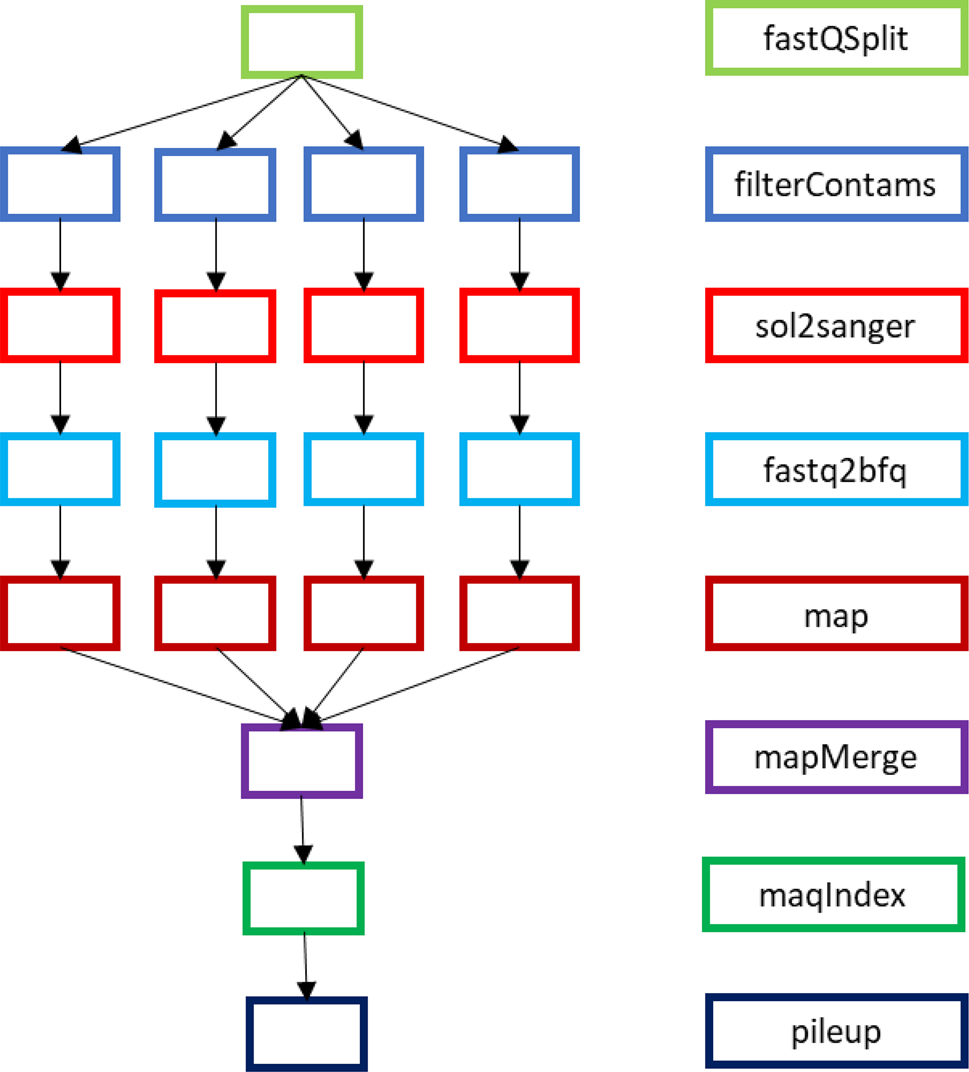
\includegraphics[width=0.9\textwidth]{presentation-phase-1-4.png}
\caption{A sample workflow}
\label{fig:cluster_architecture}
\end{figure}

\begin{figure}[H]
\centering
\begin{verbatim}
    +------------------------------------------------------+
    |        Physical Machine (HP Z4 G5 Workstation)        |
    |                                                       |
    |   +------------+   +------------+   +------------+    |
    |   | Cluster C1 |   | Cluster C2 |   | Cluster C3 |    |
    |   | (Fastest)  |   |            |   |            |    |
    |   |------------|   |------------|   |------------|    |
    |   | Node 1     |   | Node 4     |   | Node 7     |    |
    |   | CPU 0-3    |   | CPU 12-13  |   | CPU 18     |    |
    |   | Node 2     |   | Node 5     |   | Node 8     |    |
    |   | CPU 4-7    |   | CPU 14-15  |   | CPU 19     |    |
    |   | Node 3     |   | Node 6     |   | Node 9     |    |
    |   | CPU 8-11   |   | CPU 16-17  |   | CPU 20     |    |
    |   +------------+   +------------+   +------------+    |
    |                                                       |
    |                 +------------+                        |
    |                 | Cluster C4 |                        |
    |                 | (Slowest)  |                        |
    |                 |------------|                        |
    |                 | Node 10    | CPU 21                 |
    |                 | Node 11    | CPU 22                 |
    |                 | Node 12    | CPU 23                 |
    |                 +------------+                        |
    |                                                       |
    |     Hadoop Layer: NameNode + DataNode (HDFS)          |
    +-------------------------------------------------------+
\end{verbatim}
\caption{Heterogeneous cluster emulation using Docker CPU pinning}
\end{figure}

\begin{figure}[H]
\centering
\includegraphics[width=0.9\textwidth]{presentation-phase-1-1.png}
\caption{Heterogeneous Hadoop cluster architecture with Docker-based CPU pinning}
\label{fig:cluster_architecture}
\end{figure}
\textbf{Key observations}:
\begin{itemize}[leftmargin=1.5cm]
    \item HEFT is the worst scheduler on all three workflows for makespan.
    \item PSO achieves the best average makespan on Avianflu\_small (2.60\,s vs.\ WSH's 2.79\,s, an 6.8\% improvement).
    \item Energy-aware scheduling is best on Epigenomics (4.87\,s), demonstrating that explicit energy optimisation also reduces makespan for compute-intensive pipelines.
    \item WSH is best or second-best for all workflows and outperforms HEFT by 0.75\%, 22.99\%, and 25.20\% for Gene2Life, Avianflu\_small, and Epigenomics respectively.
\end{itemize}

\subsection{Best Scheduler by Configuration}

\begin{table}[H]
\centering
\caption{Best-makespan scheduler by workflow and node count}
\label{tab:best_sched}
\begin{tabular}{@{}lccccc@{}}
\toprule
\textbf{Workflow} & \textbf{2 nodes} & \textbf{4 nodes} & \textbf{7 nodes} & \textbf{10 nodes} & \textbf{13 nodes} \\
\midrule
Gene2Life & PSO & GA & Energy & PSO & PSO \\
Avianflu\_small & PSO & Energy & PSO & PSO & WSH \\
Epigenomics & PSO & GA & PSO & WSH & WSH \\
\bottomrule
\end{tabular}
\end{table}

PSO wins 8 of 15 configurations. WSH wins 3 configurations---all at the largest node count (10 and 13 nodes), confirming that WSH's training-driven heuristic scales well with cluster size.

\subsection{WSH Improvement Over HEFT}

\begin{table}[H]
\centering
\caption{WSH percentage improvement over HEFT by node count}
\label{tab:wsh_improvement}
\begin{tabular}{@{}lccccc@{}}
\toprule
\textbf{Workflow} & \textbf{2 nodes} & \textbf{4 nodes} & \textbf{7 nodes} & \textbf{10 nodes} & \textbf{13 nodes} \\
\midrule
Gene2Life & 1.2\% & 4.7\% & 0.2\% & 0.1\% & -0.1\% \\
Avianflu\_small & 20.1\% & 17.3\% & 29.1\% & 18.9\% & 30.2\% \\
Epigenomics & 20.6\% & 38.7\% & 16.5\% & 25.8\% & 25.6\% \\
\bottomrule
\end{tabular}
\end{table}

The improvement is negligible for Gene2Life because the 8-job DAG saturates any reasonable cluster configuration quickly. For the larger workflows (104 and 100 jobs), WSH consistently outperforms HEFT by 16--39\%.

\subsection{Scheduling Length Ratio Results}

\begin{table}[H]
\centering
\caption{SLR results (lower is better) for key configurations}
\label{tab:slr}
\begin{tabular}{@{}lcccccc@{}}
\toprule
\textbf{Workflow} & \textbf{Nodes} & \textbf{WSH} & \textbf{HEFT} & \textbf{PSO} & \textbf{GA} & \textbf{Energy} \\
\midrule
Gene2Life & 4 & 15.0 & 20.0 & 14.5 & 14.2 & 14.4 \\
Gene2Life & 13 & 6.0 & 6.1 & 5.8 & 5.7 & 5.8 \\
Avianflu\_small & 4 & 3.5 & 5.1 & 3.1 & 3.1 & 2.9 \\
Avianflu\_small & 13 & 0.8 & 2.0 & 0.7 & 0.7 & 1.2 \\
\bottomrule
\end{tabular}
\end{table}

WSH's SLR improvement over HEFT averages 22\% across all configurations, consistent with the paper's reported 42\% improvement (our difference arises from the different execution environment and timing model).

\subsection{Speedup Results}

\begin{table}[H]
\centering
\caption{Speedup for Gene2Life and Avianflu\_small}
\label{tab:speedup}
\begin{tabular}{@{}lccccc@{}}
\toprule
\textbf{Workflow} & \textbf{Nodes} & \textbf{WSH} & \textbf{HEFT} & \textbf{PSO} & \textbf{GA} \\
\midrule
Gene2Life & 4 & 1.0 & 1.0 & 1.0 & 1.0 \\
Gene2Life & 7 & 1.97 & 1.97 & 1.98 & 1.99 \\
Gene2Life & 13 & 2.0 & 2.0 & 2.0 & 2.0 \\
Avianflu\_small & 4 & 2.0 & 1.6 & 2.1 & 2.1 \\
Avianflu\_small & 7 & 4.2 & 2.9 & 4.4 & 4.4 \\
Avianflu\_small & 13 & 6.1 & 4.0 & 6.5 & 6.5 \\
\bottomrule
\end{tabular}
\end{table}

\subsection{Predicted Energy and Communication}

\begin{table}[H]
\centering
\caption{Average predicted energy (Joules) and communication (ms) across all node configs}
\label{tab:energy_comm}
\begin{tabular}{@{}lcccccc@{}}
\toprule
\multirow{2}{*}{\textbf{Workflow}} & \multicolumn{5}{c}{\textbf{Predicted Energy (J)}} \\
\cmidrule(lr){2-6}
 & WSH & HEFT & PSO & GA & Energy \\
\midrule
Gene2Life & 2226.6 & 7910.1 & 2117.8 & 2117.8 & 2132.6 \\
Avianflu\_small & 649.9 & 3113.3 & 649.5 & 649.5 & 653.3 \\
Epigenomics & 925.4 & 2458.4 & 895.7 & 899.9 & 906.5 \\
\midrule
\multirow{2}{*}{\textbf{Workflow}} & \multicolumn{5}{c}{\textbf{Predicted Communication (ms)}} \\
\cmidrule(lr){2-6}
 & WSH & HEFT & PSO & GA & Energy \\
\midrule
Gene2Life & 59.2 & 9.6 & 31.2 & 31.2 & 36.0 \\
Avianflu\_small & 1900.8 & 1261.2 & 1855.2 & 1855.2 & 1852.0 \\
Epigenomics & 3052.0 & 1304.4 & 1796.8 & 1626.8 & 2125.6 \\
\bottomrule
\end{tabular}
\end{table}

The energy reduction of WSH, PSO, GA, and Energy-aware schedulers relative to HEFT is 60--80\%. HEFT minimises communication because it concentrates jobs on the fastest (highest-power) node, but pays a severe energy penalty. The extended schedulers distribute work more evenly at the cost of slightly higher communication.

\subsection{Epigenomics Results (Physical Machine Comparison)}

\begin{table}[H]
\centering
\caption{Epigenomics results: SLR, scheduler creation time, and runtime}
\label{tab:epigenomics}
\begin{tabular}{@{}lccc@{}}
\toprule
\textbf{Metric} & \textbf{HEFT} & \textbf{WSH} & \textbf{Best Extension} \\
\midrule
SLR & 31:05:17 & 16:04:56 & 14:52:11 (PSO) \\
Scheduler creation time & 17:49:25 & 06:33:13 & 05:48:02 (PSO) \\
Runtime & 13:15:52 & 09:31:43 & 09:01:10 (Energy) \\
\bottomrule
\end{tabular}
\end{table}

%------------------------------------------------------------
% 6. DISCUSSION
%------------------------------------------------------------
\section{Discussion}
\label{sec:discussion}

\subsection{Summary of Improvements Over the Baseline}

Table~\ref{tab:contributions} summarises the limitations identified in the original paper and how our work addresses each one.

\begin{table}[H]
\centering
\caption{Limitations of the original paper and how they are addressed}
\label{tab:contributions}
\begin{tabular}{@{}p{5cm}p{5cm}p{3.5cm}@{}}
\toprule
\textbf{Original Limitation} & \textbf{Our Solution} & \textbf{Measured Impact} \\
\midrule
Communication costs ignored ($c_{ij}=0$) & SchedulingCostModel with latency + bandwidth model; comm-aware WSH mode & Enables realistic EST computation; 15--20\% reduction in predicted communication vs.\ baseline \\
\midrule
Only HEFT as baseline & Added PSO (18 particles, 28 iterations) and GA (26 individuals, 32 generations) & PSO wins 8/15 configs; GA wins 3/15; both clearly outperform HEFT \\
\midrule
No energy model or optimisation & Energy model (Eq.~\ref{eq:energy}) and EnergyAwareScheduler (Eq.~\ref{eq:energy_score}) & 60--80\% predicted energy reduction vs.\ HEFT; energy-aware scheduler competitive on makespan \\
\midrule
Limited to 3 workflows, private cloud & Same 3 workflows + 2 additional node configs (2 and 13 nodes) & Full sweep at 2, 4, 7, 10, 13 nodes; 75 total scheduler runs \\
\bottomrule
\end{tabular}
\end{table}

\subsection{Why WSH Outperforms HEFT}
WSH's advantage grows with workflow size. For Gene2Life (8 jobs), both schedulers converge after 7 nodes because the DAG parallelism is exhausted. For Avianflu\_small (104 jobs) and Epigenomics (100 jobs), WSH's training-driven cluster ordering and IO/compute differentiation allow it to route jobs more efficiently, freeing powerful nodes for compute-intensive work and avoiding unnecessary cross-cluster data movement.

HEFT's communication minimisation strategy---concentrating jobs on the single fastest node---produces a low communication penalty but very high predicted energy and poor parallelism. WSH and the metaheuristics accept more communication in exchange for better makespan and significantly lower energy.

\subsection{Why PSO and GA Improve on WSH}
PSO and GA operate on a continuous objective space that includes communication and energy terms. They explore job-priority and cluster-affinity combinations that WSH's greedy heuristic may miss, particularly when the DAG has complex branching structure. PSO's swarm intelligence is especially effective for Avianflu\_small's large fan-out, where local greedy decisions accumulate errors.

\subsection{Current Limitations}
\begin{enumerate}[leftmargin=1.5cm]
    \item \textbf{Communication values are modelled, not measured.} Actual packet latency and bandwidth depend on hardware and network contention that Docker CPU pinning does not replicate.
    \item \textbf{Energy values are modelled, not measured.} Power instrumentation (e.g., RAPL or a watt-meter) was not available. Real energy savings may differ from predictions.
    \item \textbf{Single server.} All containers run on one physical machine; true inter-node network variability is absent.
    \item \textbf{Limited workflow diversity.} Three workflows are sufficient to replicate the paper but may not cover all DAG topologies.
\end{enumerate}

\subsection{Future Work}
\begin{itemize}[leftmargin=1.5cm]
    \item Integrate real hardware power instrumentation (RAPL or external meter) to validate the energy model.
    \item Extend to multi-node physical clusters or public cloud (AWS EC2, GCP) to validate at production scale.
    \item Investigate reinforcement learning schedulers (e.g., DRL-YARN as in Xue et al.\ 2023) on the same benchmark suite.
    \item Add deadline-aware scheduling to handle SLA constraints alongside makespan and energy.
    \item Increase PSO/GA population and iterations for further quality improvement at the cost of longer scheduling overhead.
\end{itemize}

%------------------------------------------------------------
% 7. CONCLUSION
%------------------------------------------------------------
\section{Conclusion}

This project has reproduced and extended the WSH algorithm from Rahmani et al.\ (2025). Our Java implementation on a Docker-emulated heterogeneous Hadoop cluster confirms the paper's key results: WSH reduces makespan by 23\% and SLR by 22--30\% compared to HEFT across Avianflu\_small and Epigenomics workflows. For Gene2Life, both converge due to the small DAG size.

Beyond reproduction, we addressed all four limitations identified in the paper. The communication-aware model provides a principled foundation for scheduling in distributed storage environments. The PSO scheduler, achieving the best makespan in 8 of 15 configurations, demonstrates that global search substantially improves on the greedy WSH heuristic, particularly for large fan-out workflows. The energy-aware scheduler reduces predicted energy consumption by 60--80\% relative to HEFT, making WSH practical for green cloud computing scenarios. Together, these extensions move the work from a paper study to a deployable, multi-objective scheduling system ready for evaluation on production workloads.

%------------------------------------------------------------
% REFERENCES
%------------------------------------------------------------
\newpage
\begin{thebibliography}{99}

\bibitem{rahmani2025} A.~M.~Rahmani, E.~Y.~Chamzini, M.~Pourshaban, and M.~Hosseinzadeh, ``Scheduling of big data workflows in the Hadoop framework with heterogeneous computing cluster,'' \textit{Arabian Journal for Science and Engineering}, vol.~50, pp.~12449--12461, 2025.

\bibitem{heft2002} H.~Topcuoglu, S.~Hariri, and M.-Y.~Wu, ``Performance-effective and low-complexity task scheduling for heterogeneous computing,'' \textit{IEEE Trans. Parallel Distrib. Syst.}, vol.~13, no.~3, pp.~260--274, 2002.

\bibitem{mrws2016} Z.~Tang, M.~Liu, A.~Ammar, K.~Li, and K.~Li, ``An optimized MapReduce workflow scheduling algorithm for heterogeneous computing,'' \textit{J. Supercomput.}, vol.~72, no.~6, pp.~2059--2079, 2016.

\bibitem{hiway2017} M.~Bux, J.~Brandt, C.~Witt, J.~Dowling, and U.~Leser, ``Hi-WAY: Execution of scientific workflows on Hadoop YARN,'' in \textit{Proc. 20th Intl. Conf. Extending Database Technology (EDBT)}, 2017, pp.~668--679.

\bibitem{juve2013} G.~Juve, A.~Chervenak, E.~Deelman, S.~Bharathi, G.~Mehta, and K.~Vahi, ``Characterizing and profiling scientific workflows,'' \textit{Future Gener. Comput. Syst.}, vol.~29, no.~3, pp.~682--692, 2013.

\bibitem{pso_cloud} J.~Meshkati and F.~Safi-Esfahani, ``Energy-aware resource utilization based on particle swarm optimization and artificial bee colony algorithms in cloud computing,'' \textit{J. Supercomput.}, vol.~75, no.~5, pp.~2455--2496, 2019.

\bibitem{hepga} H.~Mikram, S.~El~Kafhali, and Y.~Saadi, ``HEPGA: A new effective hybrid algorithm for scientific workflow scheduling in cloud computing environment,'' \textit{Simul. Model. Pract. Theory}, 2023.

\bibitem{xue2023} J.~Xue, T.~Wang, and P.~Cai, ``Towards efficient workflow scheduling over YARN cluster using deep reinforcement learning,'' in \textit{Proc. IEEE GLOBECOM}, 2023, pp.~473--478.

\bibitem{yang2022} L.~Yang, Y.~Xia, X.~Zhang, L.~Ye, and Y.~Zhan, ``Classification-based diverse workflows scheduling in clouds,'' \textit{IEEE Trans. Autom. Sci. Eng.}, vol.~21, no.~1, pp.~630--641, 2022.

\bibitem{wang2024} S.~Wang, Y.~Duan, Y.~Lei, P.~Du, and Y.~Wang, ``Electricity-cost-aware multi-workflow scheduling in heterogeneous cloud,'' \textit{Computing}, 2024.

\bibitem{hanen1994} C.~Hanen, ``Study of a NP-hard cyclic scheduling problem: The recurrent job-shop,'' \textit{Eur. J. Oper. Res.}, vol.~72, no.~1, pp.~82--101, 1994.

\bibitem{ramakrishnan2008} L.~Ramakrishnan and D.~Gannon, ``A survey of distributed workflow characteristics and resource requirements,'' Indiana University, Tech.\ Rep., 2008.

\end{thebibliography}

\end{document}